\chapter[Motores de Juego]{\label{identificadorReferenciaCruzada}
Motores de Juego}


Un motor de juego, es una herramienta software diseñada para asistir a los desarrolladores en la tarea de creación de juegos y aplicaciones gráficas\cite{B9}.

\section{Arquitectura:}

Un motor de juego está compuesto por una capa de tarjeta Hardware que representa el pc o consola sobre el que se ejecutará, una capa de drivers que son componentes Software que proporciona el sistema operativo o el proveedor de HArdware.

Por otra parte tiene el sistema operativo sobre el que está ejecutándose el juego todo el tiempo, la parte de SDKs que da soporte a la parte de programación del juego y la parte de estructuras de datos y algoritmos para dar soporte a la programación también.

Si nos centramos en la parte estética del juego, nos encontramos con una parte gráfica, una parte de animación de personajes y modelos y una parte de colisiones y física en la que se deforman los escenarios y da realismo al juego.

Sin embargo, si nos fijamos en la parte de la inteligencia artifical, nos encontramos una parte dedicada especialmente a eso, que está producida por el SDK.

Por último nos encontramos una serie de capas que ayudan a la depuración, renderizado, efectos visuales y gameplay para realizar pruebas.

En la \ref{Figura3} podemos ver como se organizan las distintas partes.

\begin{figure}[h!]

	\centering
	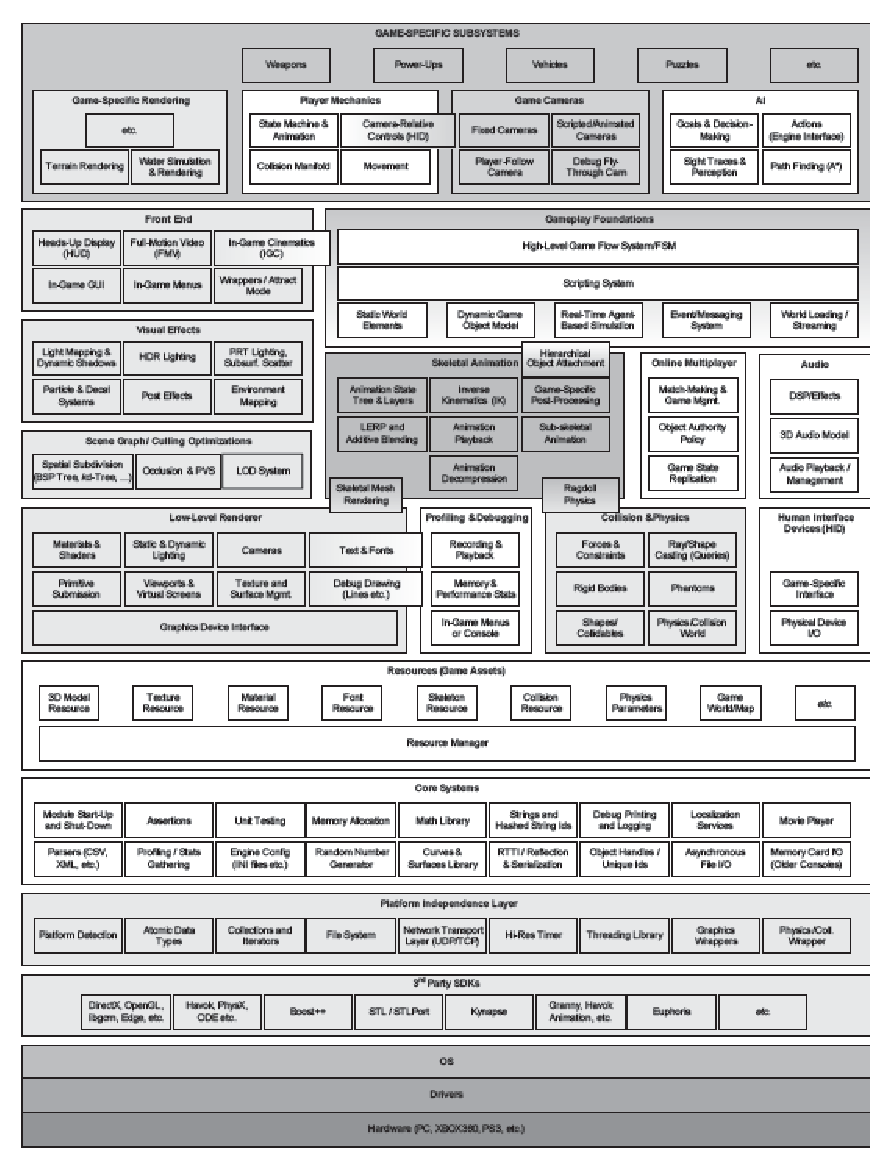
\includegraphics[width=8cm]{./eps/fig3.eps}
	\caption{Arquitectura de un motor de juegos, extraído de \cite{B10}}
	\label{Figura3}

\end{figure}
\newpage

\section{Selección de motor:}
Hay cientos de motores gráficos en el mercado y a la hora de elegir uno para el desarrollo de un proyecto hay que tener en cuenta los siguientes criterios\cite{B9}:

\begin{itemize}

	\item Si la herramienta tiene soporte o no para 2D y 3D.
	\item Si la herramienta es multiplataforma.
	\item Los lenguajes de programación que soporta la herramienta.
	\item Si tiene un motor de físicas y herramientas de inteligencia artificial.
	\item Si incorpora herramientas más avanzadas como editores de terrenos.
	\item El tipo de licencia que utiliza. 

\end{itemize}

En la tabla \ref{Tabla3} están los tres motores de juegos más importantes del mercado.

\begin{sidewaystable}[hbp]
\resizebox{20cm}{!}{ 
\begin{tabular}{| p{2cm} | p{1.5cm} | p{1.5cm} | p{2.5cm} | p{2cm} | p{2cm} | p{2cm} | p{4cm} | p{3.5cm}|}
	\hline 
		Nombre & 2D/3D & IDE & Lenguaje & Plataforma & Motor Físico & Herramientas de IA & Características Avanzadas & Licencia\\
   		\hline 
   		Unity3D & 2D y 3D & Mac y Windows & C\#, Boo, JS & Mac, Windows,
   		Linux, iOS, Android, PS3, XB360, PSP, Wii, PSVita, Flash,
   		Web & PhysX &  NavMesh y Path Finding & Forward y Deferred
   		rendering, Occlusion Culling, light mapping, light probing, LOD discreto, edición de terrenos, sistema de partículas & Comercial. Versión básica
   		gratuita (desktop y web) y versiones PRO y plataformas
   		móviles y consolas con un pago único sin royalties\\
   	\hline
    	UDK/Unreal Engine 4& 2D y 3D & Sí & Unreal Script & Mac, Windows,
    	iOS, Android, PS3, XB360, PSVita, Wii, Flash & PhysX &Path Finding &  Deferred rendering, occlusion culling, parallax mapping, Per Object Motion
    	Blur  &  Comercial. Versión libre y pago de royalties sobre producto vendido al superar un umbral de facturación. La versión Unreal Engine 3 dispone de más funcionalidades y una licencia comercial más cara.\\
    \hline
        Corona SDK & 2D & No & LUA & iOS, Android, Nook, Kindle Fire & Box2D & No. Deben ser programadas desde cero en LUA  & Interfaz simple de Lua para
        la programación de física & Comercial. Versión Indie para desarrollar para una única plataforma (iOS o Android) y versión Pro para todas las
        plataformas.\\
    \hline
\end{tabular}
}


\caption{Lista de Motores obtenida en el artículo: \cite{B9}} \label{Tabla3}
\end{sidewaystable}

Una vez que sabemos los criterios y los motores más usados del mercado, podemos disponernos a elegir un motor para nuestro proyecto.

Como el proyecto, tiene una parte en 2D, que es la de generación de planetas, necesitamos un motor que disponga de 2D, los cuales son los tres, sin embargo la parte de generación de ciudades, se hará en 3D, por lo que será necesario que disponga de 3D también,por lo que descartaremos el Corona SDK.

Por otra parte, necesitamos algo que se haga en PC, así que nos sirven los dos motores que nos quedan, pero si nos fijamos en los lenguajes de programación, Unity tiene una mayor variedad respecto a UDK que sólo soporta ''Unreal script''.

Si nos fijamos en la parte de motor de físicas, que es un motor que simula los movimientos físicos \cite{B11}, vemos que es una parte irrelevante, ya que no vamos a mover nada, ni vamos a generar movimientos sismicos, ni de personajes.

Por otra parte si nos fijamos en la parte de la inteligencia artificial, vemos que Unity tiene una mayor variedad que UDK, lo que para el proyecto nos beneficia bastante para la programación de los algoritmos genéticos, lo mismo que pasa con las características avanzadas.

Si nos fijamos en el punto de licencias, Unity cuenta con una versión gratuita para la plataforma de PC, lo que nos viene perfecto, sin embargo, UDK para ofrecernos lo mismo que Unity requiere de una subcripción.

Una vez estudiado todas las características que nos proporcionan los motores que más se usan en el mercado, podemos decir que Unity es el que más nos beneficiará para el desarrollo del proyecto.


\newpage




